%% Owner: Mikael Rodriguez
\section{Stack: stats}
\label{sec:stats}
The stats stack provides monitoring for the Docker Swarm cluster.
Prometheus collects and stores metrics, while Grafana displays them
in dashboards. Node Exporter collects host metrics and cAdvisor
collects container metrics. This allows us to monitor resource usage
and check that metrics are available across the cluster.

\subsection{Services and images}
The stack uses four services, listed in \Cref{tab:services}.
\begin{table}[htbp]
\centering
\caption{Services of the stats stack.}
\label{tab:services}
\small
\begin{tabular}{l>{\raggedright\arraybackslash}p{48mm}>{\raggedright\arraybackslash}p{60mm}}
\toprule
Service & Image & Role \\
\midrule
Prometheus & Official Prometheus image
& Scrapes and stores metrics from the exporters \\
Grafana & Custom Grafana image
& Displays metrics in dashboards and includes the required
datasource plugin \\
Node Exporter & Official Prometheus Node Exporter image
& Exposes CPU, memory, disk and network metrics from
the host \\
cAdvisor & Official cAdvisor image
& Exposes resource usage metrics for Docker containers \\
\bottomrule
\end{tabular}
\end{table}

Prometheus scrapes Node Exporter on port 9100 and cAdvisor on port
8080. Grafana uses the Prometheus datasource at
\texttt{http://prometheus:9090} to query the collected metrics.

\subsection{Dockerfiles}
Only Grafana requires a custom Dockerfile. It extends the official
Grafana image and installs the plugin needed by the project. Building
this image ensures that the plugin is available whenever the service
starts, without having to install it manually through the Grafana
interface.

The other services use official images. Their configuration is supplied
through the Compose files and Prometheus configuration.

After changing the Dockerfile or plugin version, the Grafana image
must be rebuilt and published to the registry before deploying the
updated image to the Swarm.

\subsection{\texttt{compose.yml} and \texttt{production.yml}}
The local Compose file is used to test monitoring on a developer
machine, while \texttt{production.yml} deploys the services on Swarm.
The main differences are shown in \Cref{tab:diff}.
\begin{table}[htbp]
\centering
\caption{Differences between local and production monitoring.}
\label{tab:diff}
\small
\begin{tabular}{>{\raggedright\arraybackslash}p{28mm}>{\raggedright\arraybackslash}p{49mm}>{\raggedright\arraybackslash}p{51mm}}
\toprule
& \texttt{compose.yml} & \texttt{production.yml} \\
\midrule
Deployment & Local Docker Compose
& Docker Swarm stack \\
Images & Local or published images
& Published images available to Swarm nodes \\
Discovery & Compose service names
& Docker DNS discovery of Swarm tasks \\
Networking & Compose network
& Overlay network \texttt{monitoring\_backend} \\
Configuration & Local files and mounts
& Swarm configs and production settings \\
Placement & Local machine
& Services placed according to Swarm constraints \\
Storage & Local volumes
& Production volumes or host paths, as configured \\
\bottomrule
\end{tabular}
\end{table}

In production, Prometheus discovers exporter tasks through DNS:
\texttt{tasks.monitoring\_node-exporter} and
\texttt{tasks.monitoring\_cadvisor}. This avoids maintaining a static
list of task IP addresses and allows Prometheus to discover tasks as
they change.

\subsection{Replicas, placement and update policy}
Each monitoring service runs one replica. Prometheus and Grafana are
placed on \texttt{swarm-manager-1}, which provides a predictable
location for the central monitoring services. This also aligns with
the node used to access Grafana through the nginx reverse proxy.

Placement constraints and local storage requirements must be
considered when rescheduling these services.

Node Exporter and cAdvisor run on the Swarm nodes to expose host and
container metrics. Prometheus discovers their tasks through the
\texttt{monitoring\_backend} overlay network.

With one replica, restarting or updating Prometheus or Grafana can
temporarily interrupt monitoring. Updates must use the image and
configuration versions defined in the production stack file.

\subsection{Volumes, NFS paths and secrets}
Prometheus needs persistent storage if collected time-series data
must survive container replacement. Grafana may also use persistent
storage for data maintained inside Grafana. The exact volume mounts
are defined in the stack configuration.

The \texttt{monitoring\_backend} overlay network allows Prometheus
to reach the exporters and Grafana to reach Prometheus by service
name. Node Exporter and cAdvisor also expose ports 9100 and 8080
in the configured deployment, but their metrics should not be
published publicly without a reason.

Grafana's administrator password must be configured securely rather
than committed to the repository. For local testing, create a password
in an environment file excluded from Git, or supply it through the
local environment. In production, use the secret or environment
mechanism defined by the deployment configuration. Do not put real
passwords in the Compose files or documentation.

For example, generate a strong password locally with:
\begin{shell}
openssl rand -base64 24
\end{shell}

Store the generated value in the appropriate local environment file
or production secret. Restrict access to the file and ensure it is
excluded from version control. If the configuration uses a Swarm
secret, create it before deploying the stack and reference its
actual name in \texttt{production.yml}.

\subsection{Health checks and metrics}
Prometheus scrapes the exporters every 15 seconds. Node Exporter
provides host-level metrics, while cAdvisor provides container-level
metrics. Grafana uses these measurements to display CPU, memory,
disk, network and container usage.

The Prometheus Targets page shows whether each exporter is being
scraped successfully. Grafana dashboards provide a visual overview
of the collected metrics. These checks are separate from Docker
health checks: a running container does not necessarily mean that
Prometheus can scrape its metrics.

\subsection{Testing}
\paragraph{Locally.}
Start the local monitoring stack and check the containers:
\begin{shell}
docker compose -f stats/compose.yml up -d
docker compose -f stats/compose.yml ps
docker compose -f stats/compose.yml logs prometheus
\end{shell}

Open Grafana at the address and port configured in
\texttt{compose.yml}. Log in using the local administrator credentials.
Check that the Prometheus datasource is working, then open the
Prometheus Targets page and confirm that the configured targets are
healthy.

If the local configuration publishes Prometheus on port 9090, its
targets page can be opened at:
\begin{shell}
http://localhost:9090/targets
\end{shell}

Check that the dashboards display data rather than empty graphs.
The local dashboard is shown in \Cref{fig:local-dashboard}.
\begin{figure}[htbp]
\centering
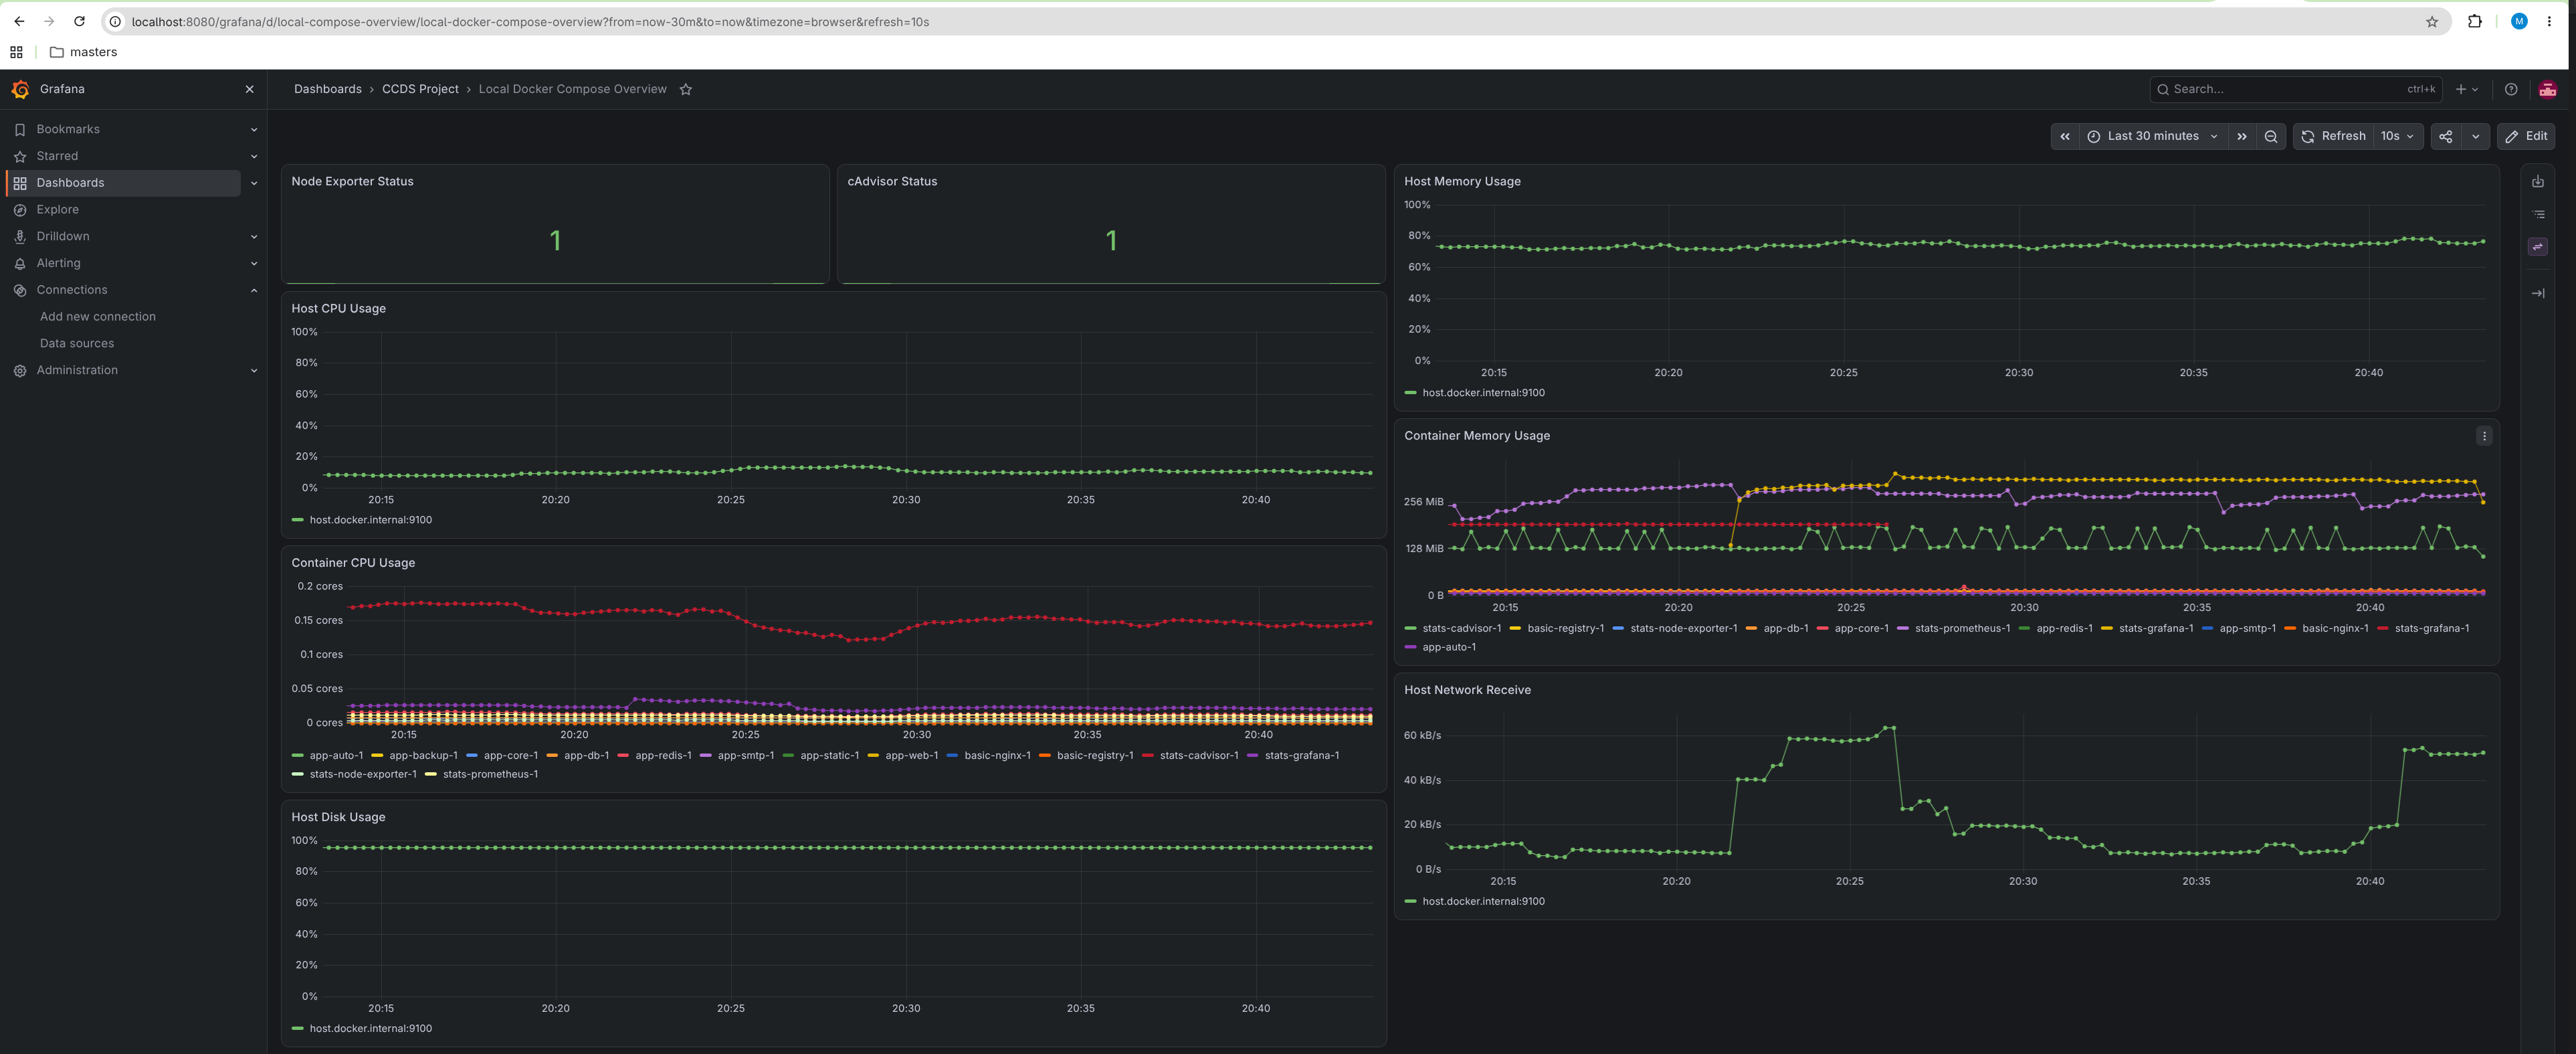
\includegraphics[width=\textwidth]{figures/local-dashboard.png}
\caption{Grafana dashboard for local Compose monitoring.}
\label{fig:local-dashboard}
\end{figure}

\paragraph{On the Swarm.}
Deploy the production stack and inspect the services and logs:
\begin{shell}
sudo docker stack deploy -c stats/production.yml monitoring
sudo docker stack services monitoring
sudo docker service ps monitoring_prometheus
sudo docker service ps monitoring_grafana
sudo docker service logs monitoring_prometheus
\end{shell}

Check that the services have the expected replica counts. In
Prometheus, verify that the Node Exporter and cAdvisor targets are
healthy and that metrics are being collected from the Swarm nodes.
Then open Grafana through the configured nginx URL and confirm that
the provisioned dashboard displays current data.

The production dashboard is shown in \Cref{fig:production-dashboard}.
\begin{figure}[htbp]
\centering
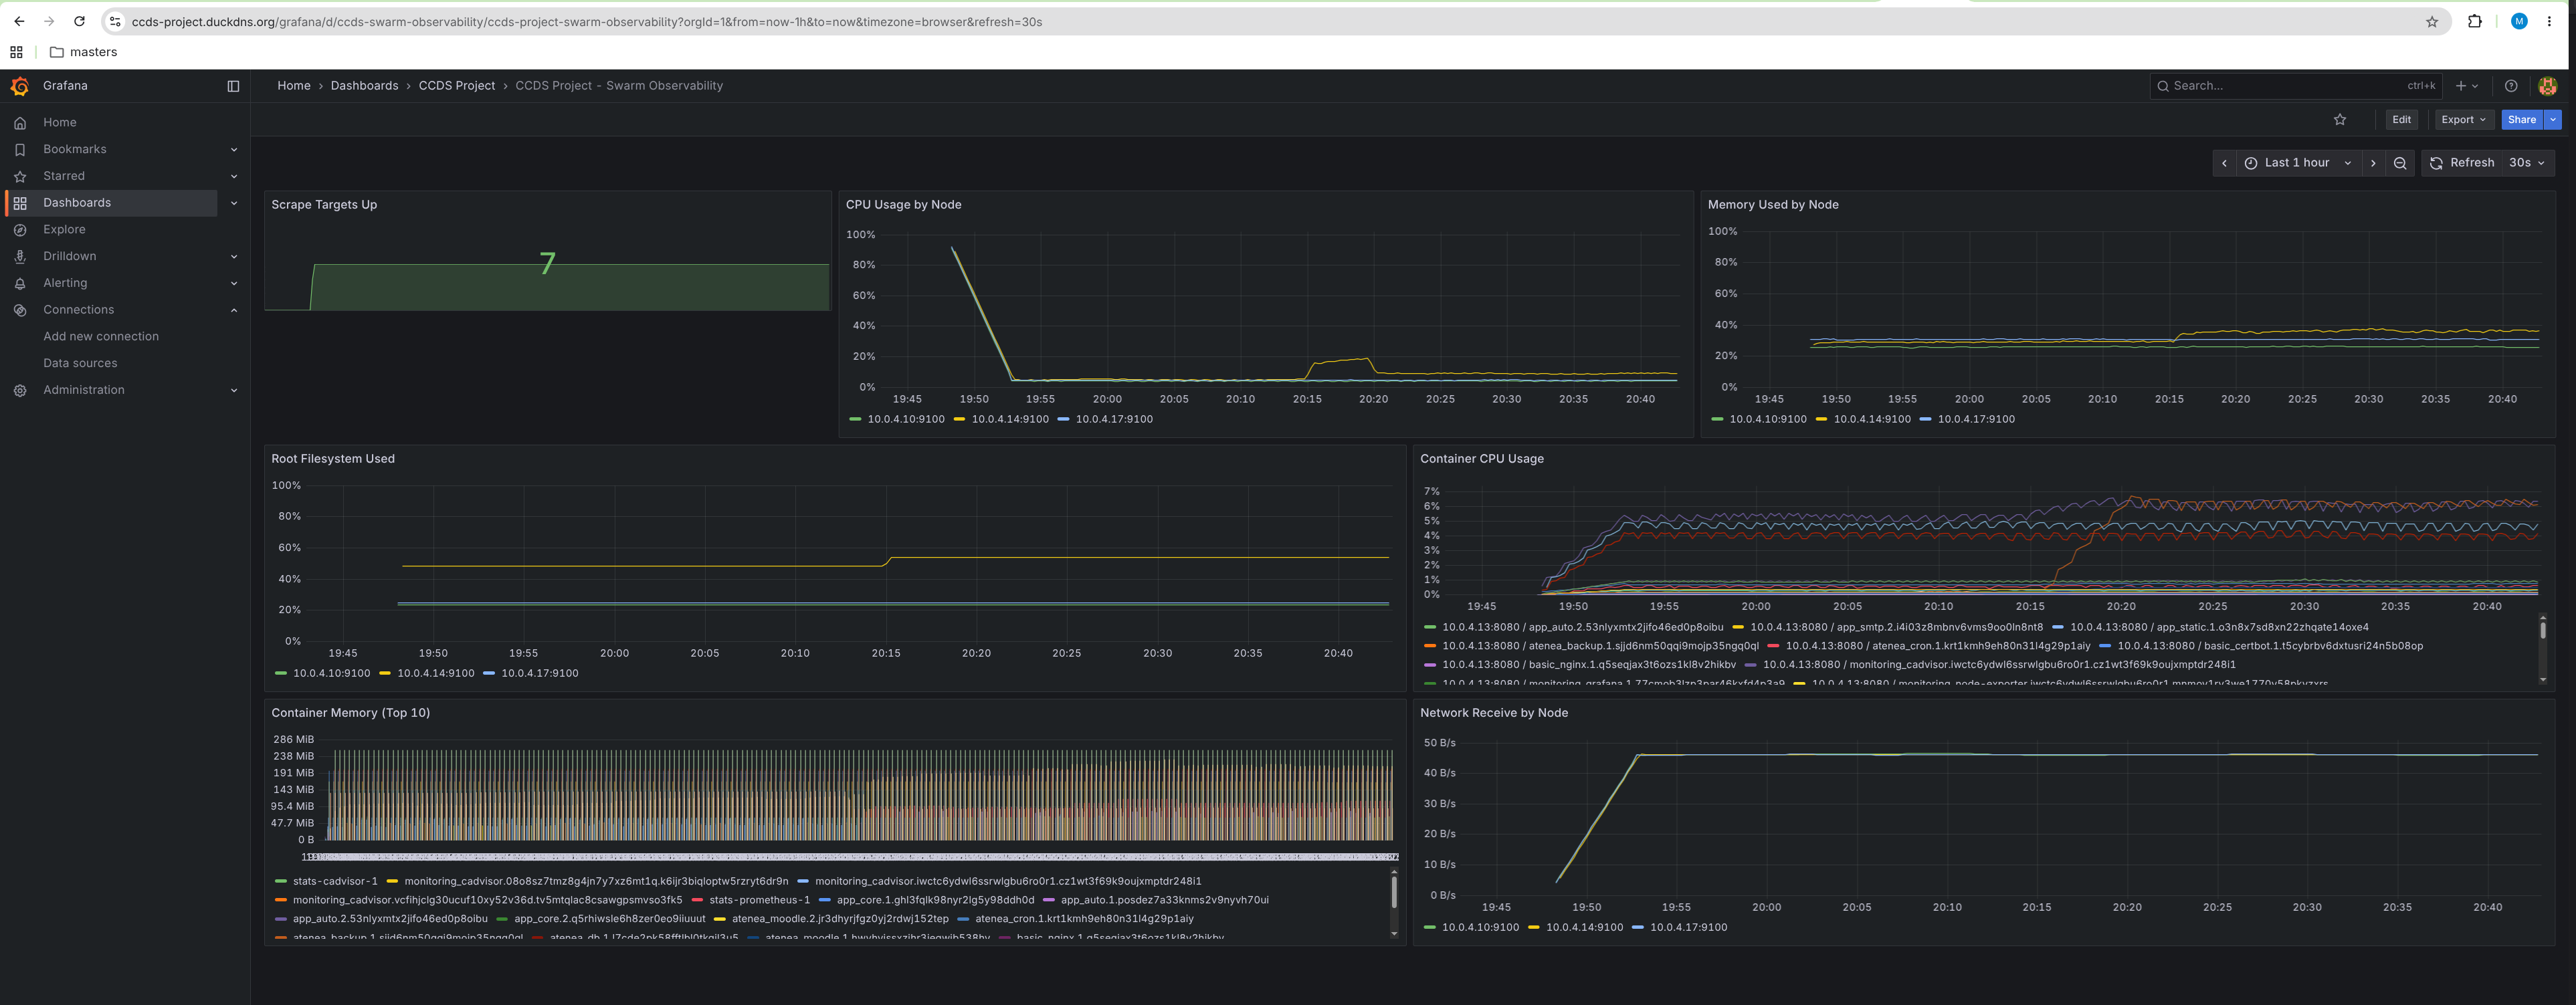
\includegraphics[width=\textwidth]{figures/production-dashboard.png}
\caption{Grafana dashboard for Swarm production monitoring.}
\label{fig:production-dashboard}
\end{figure}

Finally, verify that monitoring continues to work after restarting
a service and that the dashboards recover when Prometheus becomes
available again. Record the actual results of these tests.
